For å diskretisere sirkelen konstruerer vi to \texttt{linspace}, nemlig $\theta_{\mathtt{p}}$ og $\theta_{\mathtt{m}}$, for å så lage to tupler med punkter som ligger på sirkelen.
Vi definerer dem på følgende vis.
\[
    \theta_{\mathtt{p}} = \mathtt{linspace}\left(\frac{2\pi}{\mathtt{N}}, 2\pi, \mathtt{N}\right)
\]
\[
    \theta_{\mathtt{m}} = \mathtt{linspace}\left(0, \frac{2\pi(\mathtt{N} - 1)}{\mathtt{N}}, \mathtt{N}\right)
\]
Her er $\mathtt{N}$ antall noder.
Vi kan nå definere punkter på sirkelen ved å definere $\xtt = R_0(\cos{\theta}, \sin{\theta})$, for både $\theta_{\mathtt{p}}$ og $\theta_{\mathtt{m}}$.
Vi ser at $\theta_{\mathtt{m}}$ er etterslepende, fordi vi da kan finne midtpunktet ved å ta gjennomsnittet mellom dem.
Det er i disse midtpunktene vi vil evaluere $\phi$.

Det er hensiktsmessig å lage en klasse for å løse intergrallikningen, og midtpunktene bør være en metode her.
Vi definerer dermed klassen \texttt{IntegralEquation} i filen \texttt{integralequation.py}.
Vi har da metoden \zhett $\rightarrow$ \texttt{tuple}, som er definert ved $\zhett = \sfrac{1}{2}(\xtt_{\mathtt{p}} + \xtt_{\mathtt{m}})$.
For å sette sammen venstre side av integrallikningen, trenger vi en metode for å konstruere $\Thetatt \in \mathbb{R}^{\mathtt{N}\times\mathtt{N}}$.
Vi gjør dette med \texttt{for}-løkker over indeksene \texttt{i} og \texttt{j}.
\begin{algorithm}[H]
    \caption{Assemble $\Thetatt$}\label{alg:theta}
    \begin{algorithmic}
        \For{$\mathtt{i},\mathtt{j} \leq \mathtt{N}$}
            \If{$\mathtt{i} = \mathtt{j}$}
                \State $\Thetatt_{ij} \gets -\pi$
            \Else
                \State $\textit{\texttt{a}}_{\mathtt{p}}, \textit{\texttt{a}}_{\mathtt{m}} \gets \xtt_{\mathtt{p}} - \zhett, \xtt_{\mathtt{m}} - \zhett$
                \State $\texttt{argument} \gets \frac{\textit{\texttt{a}}_{\mathtt{p}} \cdot \textit{\texttt{a}}_{\mathtt{m}}}{\absl{\textit{\texttt{a}}_{\mathtt{p}}} \absl{\textit{\texttt{a}}_{\mathtt{m}}}}$
                \State $\Thetatt_{ij} \gets -\arccos{(\texttt{argument})}$
            \EndIf
        \EndFor
    \end{algorithmic}
\end{algorithm}

\noindent Grunnet maskinregningsfeil, kan \texttt{argument} ende opp med verdier litt høyere enn 1, si $1 + \epsilon$, hvor vi typisk får at $\epsilon = O(10^{-8})$.
Som en følge, vil Numpy vise en feilmelding i \texttt{numpy.arccos}.
Ved å legge inn en toleranse, unngår vi feilmeldingen, og koden kompilerer.
Toleransen bør sjekkes slik at man både ser at avviket er mindre enn toleransen \emph{og} at argumentet faktisk er større enn $1$.

For å regne ut høyresiden av integrallikningen, må vi sette sammen matrisen \texttt{h}.
Den inneholder en tilnærming av integralet til logaritmefunksjonen over sirkelbuen mellom $\xtt_{\mathtt{p}}$ og $\xtt_{\mathtt{m}}$.
Denne tilnærmingen er gjort med en to-punkts \textsc{Gauss}kvadraturmetode.
Utledningen og referanser er å finnes i forelesningsnotatene.
Denne matrisen skal skalarmultipliseres med moden vi er ute etters normalvektor.
Vi lager en metode som finner normalvektoren.
Siden alle normalvektorene ligger på todimensjonale linjestykker, vil normalvektoren være gitt ved $\mathtt{\hat{n}} = \absl{(\mathtt{\Delta} \xtt, \mathtt{\Delta} \ytt)}^{-1}(-\mathtt{\Delta}\textit{\texttt{y}}, \mathtt{\Delta}\xtt)$.
Vi lager en metode som setter sammen høyresiden av likningen, slik at løsningen kan finnes med \texttt{numpy.linalg.solve}.

I en ny fil kan vi konstruere koordinatene for en sirkel, og finne addert masse.
I figur \ref{fig:added_mass_circle}, ser vi at den teoretiske adderte massen i sjette mode er identisk oppfylt.
Dette er grunnet definisjonen på normalvektoren på en sirkelgeometri---den samsvarer med posisjonsvektoren, så deres kryssprodukt blir null.
Konvergensen til den adderte massen i første og andre mode er relativt god.
Ser man på verdiene, virker det som en dobling i $N$ vil føre til en reduksjon i relativ feil på faktor fire.
\begin{Figure}
    \centering
    \captionsetup{type = figure}
    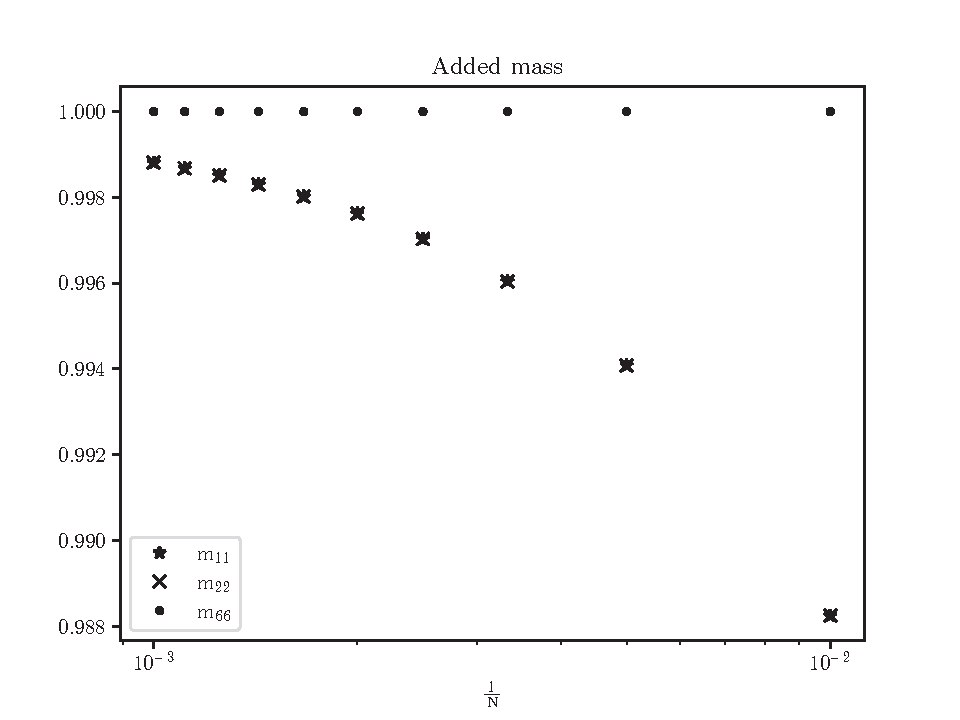
\includegraphics[width = \linewidth]{SECTIONS/CIRCLE/addedmass_circle_N1000.pdf}
    \captionof{figure}{Numerisk utregnet over teoretisk addert masse på en sirkel.}
    \label{fig:added_mass_circle}
\end{Figure}
\noindent Første modes potensial kan vi finne analytisk, som sett i første forelesningsnotat.
\[
    \phi_1 = - {R_0}^2 \deex \ln{r} = -\cos{\theta},
\]
når vi er på randa til enhetssirkelen.
Samsvaret mellom analytisk og numerisk løsning er utmerket for høye verdier av N, som vi ser i figur \ref{fig:phi1_N250}.
\begin{Figure}
    \centering
    \captionsetup{type = figure}
    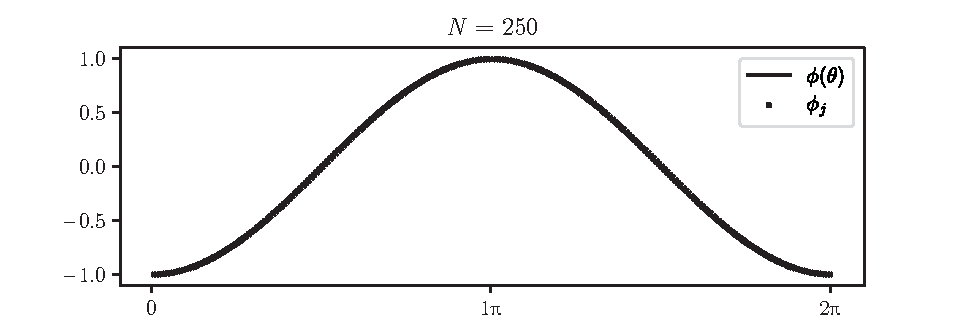
\includegraphics[width = \linewidth]{phi1_N250.pdf}
    \captionof{figure}{$\phi_1$ er gitt analytisk med heltrukket linje, og numerisk med punkter.}
    \label{fig:phi1_N250}
\end{Figure}
Vi kan finne feilen i den numeriske løsningen ved å sjekke $L^2$-normen:
\[
    {\left( {\Vert \phi_j - \phi(\theta) \Vert}_{L^2} \right)}^2 = \int_{\Omega} {\left( \phi_j - \phi(\theta) \right)}^2 \,\dee x.
\]
Vi ser at den numeriske løsningen allerede blir veldig god når vi kun har 100 noder på sirkelen.
\begin{center}
\begin{tabular}{|c|c|c|}
    \hline
    $N$ & $\phi_1$ feil & $\phi_2$ feil\\\hline
    10 & .547075 & .501985\\\hline
    20 & .285168 & .272773\\\hline
    30 & .192806 & .187301\\\hline
    40 & .145664 & .142582\\\hline
    50 & .117055 & .115091\\\hline
    60 & .097843 & .096484\\\hline
    70 & .084050 & .083054\\\hline
    80 & .073666 & .072906\\\hline
    90 & .065566 & .064967\\\hline
    100 & .059072 & .058587\\\hline
\end{tabular}
\end{center}

\noindent Andre modes potensial kan vi også finne analytisk på samme vis som første modes, dog med deriverte i $y$.
Vi har altså at $\phi_2 = -\sin{\theta}$.
\begin{Figure}
    \centering
    \captionsetup{type = figure}
    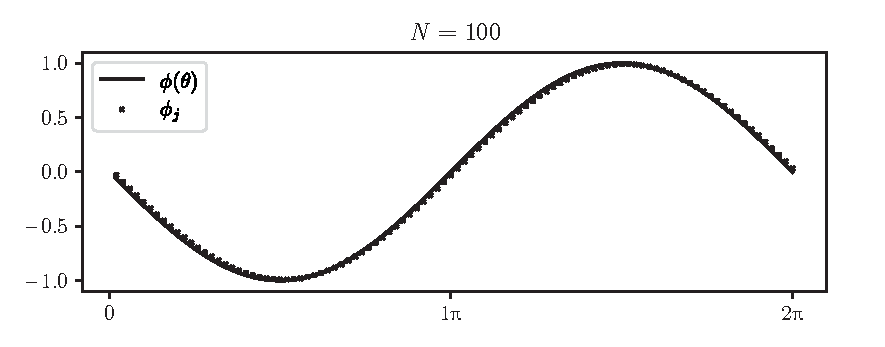
\includegraphics[width = \textwidth]{phi2_N100.pdf}
    \captionof{figure}{$\phi_2$ er gitt analytisk med heltrukken linje, og numerisk med punkter.}
    \label{fig:phi2_N100}
\end{Figure}

\noindent Vi formoder at sjette modes potensial er identisk lik null---vi har ingen heft, så rotasjonen av en rotasjonssymmetrisk geometri bør ikke forflytte fluid.
Den numeriske utregningen vår sier seg enig i dette, som sett i figure \ref{fig:phi6_N100}.
\begin{Figure}
    \centering
    \captionsetup{type = figure}
    \includegraphics[width = \textwidth]{phi6_N100.pdf}
    \captionof{figure}{$\phi_6$ er gitt numerisk med punkter.}
    \label{fig:phi6_N100}
\end{Figure}